\section{Problem 1}

The first problem issues a Low Voltage Differential Signaling line as showed in figure \ref{lvds}. The LVDS technology is a high speed ($> 155.5 Mbps$), lower power general purpose interface standard that solves the physical layer bottleneck problems related to higher data rates. According to Texas Instruments "An Overview of LVDS Techonology", its characteristics are:

\begin{itemize}
    \item LVDS uses differential data transmission that overcomes the problem related to common mode noise in single-ended schemes;
    \item LVDS features a low voltage swing compared to other industry data transmission standards;
    \item LVDS uses a constant current mode driver and the transmission media must be terminated to its characteristic impedance to prevent reflections;
    \item And many others.
\end{itemize}


\begin{figure}[H] 
\centering
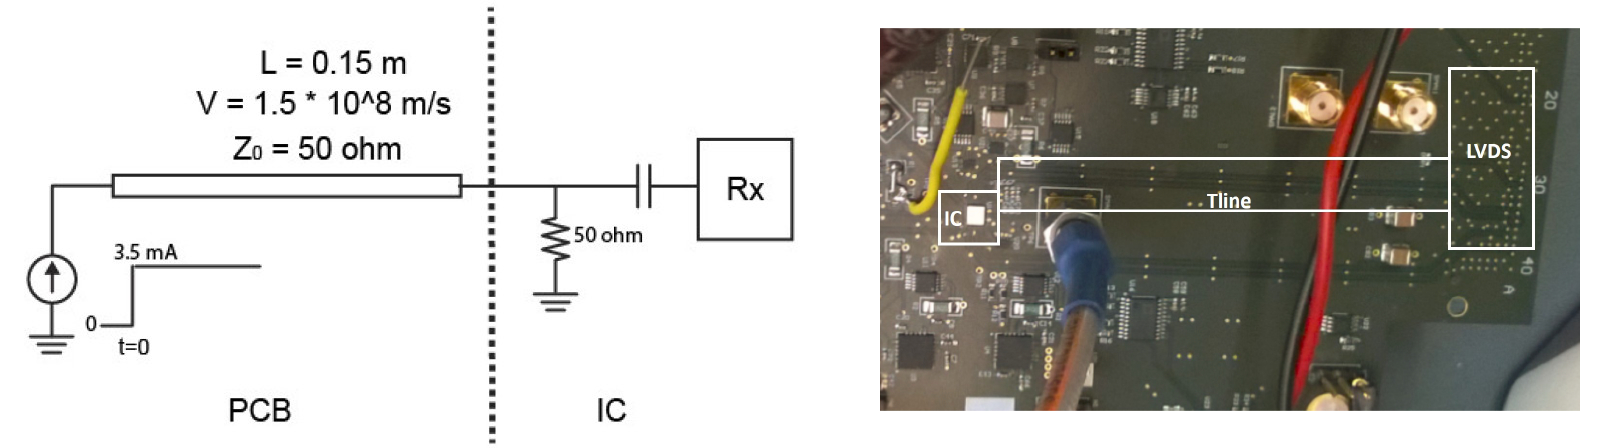
\includegraphics[width=14cm]{images/lvds.png}
\caption{LVDS.}
\label{lvds} 
\end{figure}

\subsection{Load voltage with impedance match}

Considering the transmission line in the schematic of figure \ref{lvds}, we can define the load impedance as $Z_L = 50 \Omega$ and the line characteristic impedance as $Z_0 = 50 \Omega$. The load is matched with the line since their impedance are both equal. This means that any wave travelling from the source will be fully absorbed by the load and therefore there will not be any reflected wave back to the source.

At $t=0$ the line current is only the parcel of the incident current with value determined by the source step current, so $I = I^+ + I^- = I^+ = 3.5 mA$, since it had no time to travel through the line and perhaps be reflected.

The line length is $l = 0.15m$ and the wave propagation velocity in the medium is $v = 1.5 10^{8} m/s$. So the time for any wave to propagate from one end to another of the line is $t = \frac{l}{v} = 1 ns$.

The voltage at the source end of the line will see only the line impedance. But the voltage at the load end of the line will only encounter the incident current within one propagation period ($1ns$). So the incident voltage wave will be: $V^+ = Z_L I^+ = 175 mV$.


\begin{figure}[H]
\centering

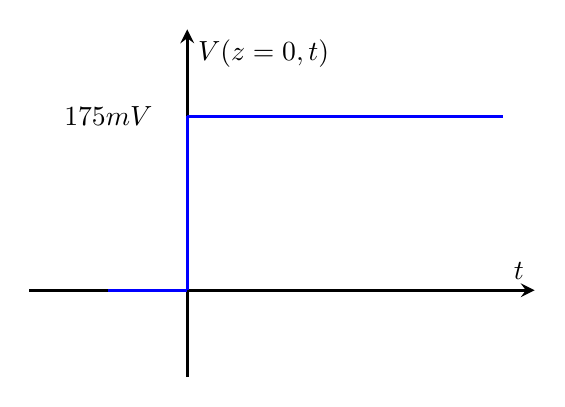
\begin{tikzpicture} 
\begin{axis}[very thick,
                     samples = 100,
                     ytick={-2,2},
                     xlabel = {$t$},
                     ylabel = {$V(z=0, t)$},
                     xmin = -1,
                     xmax = 2.2,
                     ymin = -0.5,
                     ymax = 1.5,
                     width=8cm,
                     height=6cm,
                     axis x line = middle,
                     axis y line = middle,
                     ticks = none]
                     
            \addplot[blue] coordinates {(-0.5,0) (0,0)};
            \addplot[blue] coordinates {(0,0) (0,1)};
            \addplot[blue] coordinates {(0,1) (2,1)};
            \node at (axis cs:-0.5,1){$175 mV$};
            
        \end{axis}
\end{tikzpicture}

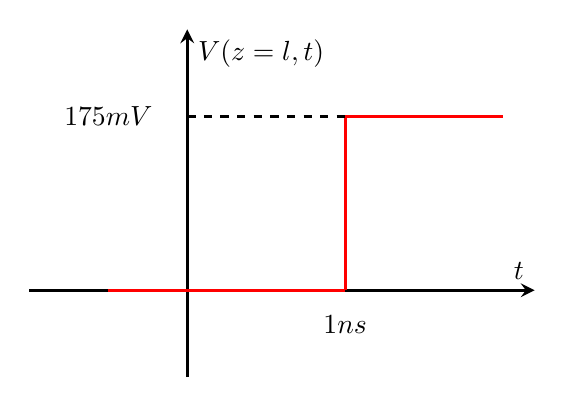
\begin{tikzpicture} 
\begin{axis}[very thick,
                     samples = 100,
                     ytick={-2,2},
                     xlabel = {$t$},
                     ylabel = {$V(z=l, t)$},
                     xmin = -1,
                     xmax = 2.2,
                     ymin = -0.5,
                     ymax = 1.5,
                     width=8cm,
                     height=6cm,
                     axis x line = middle,
                     axis y line = middle,
                     ticks = none]
                     
            \addplot[red] coordinates {(-0.5,0) (1,0)};
            \addplot[red] coordinates {(1,0) (1,1)};
            \addplot[red] coordinates {(1,1) (2,1)};
            \addplot[dashed] coordinates {(0,1) (1,1)};
            \node at (axis cs:-0.5,1){$175 mV$};
            \node at (axis cs:1,-0.2){$1ns$};
            
        \end{axis}
\end{tikzpicture}

\caption{First graph shows the voltage at the start of the line and the second shows the voltage at the end of the line. Source: own.}
\label{graph:1} 
\end{figure}

Once $Z_L = Z_0$, the expression for the reflected voltage wave in equation \ref{gamma} results in $V^-= 0$. So indeed there is no reflected wave.

\begin{equation} \label{gamma}
    \frac{V^-}{V^+} = \frac{Z_L - Z_0}{Z_L + Z_0} = \Gamma
\end{equation}

Simulating the circuit via ADS we easily confirm the theoretical wave forms from the figure \ref{graph:1} by the plot of figure \ref{ads:plot:voltages50}

\begin{figure}[H] 
\centering
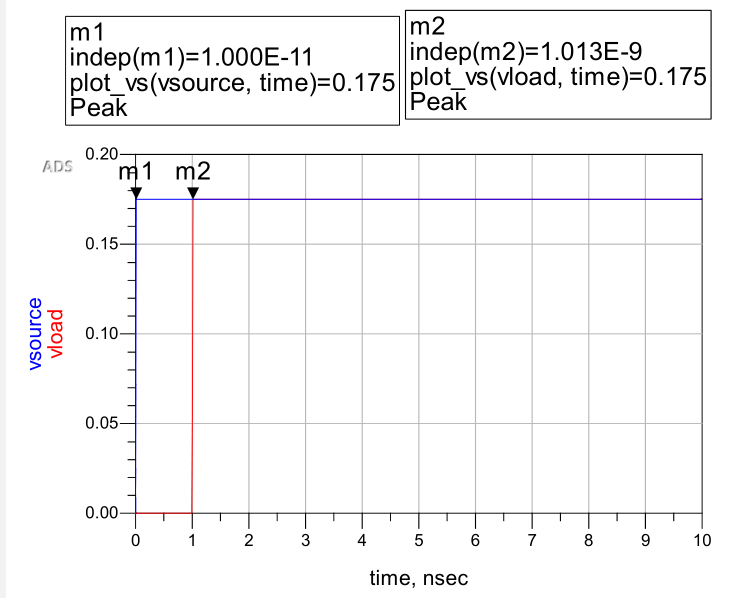
\includegraphics[width=9cm]{images/lab1_p1_plot1.png}
\caption{ADS plot of voltage values in each end of the line for: $Z_L = 50 \Omega$, $Z_0 = 50 \Omega$ and $Z_S = \infty$.}
\label{ads:plot:voltages50} 
\end{figure}

\subsection{Steady-state load voltage with impedance mismatch}

Considering a characteristic line impedance different from the load impedance ($Z_0 \neq 50 \Omega$), according to equation \ref{gamma} the reflected voltage wave will not be null anymore. Even so evaluating successive reflections in both ends of the line due to the impedance mismatch  at a time $t=\infty$ the line will not have effect in the transmission, so the voltage at the load end of the line at $t=\infty$ is: $V(z=l, \: t=\infty) = Z_L I = 50 \times 3.5 \times 10^{-3} = 175mV$.

\subsection{Load voltage waveform for $Z_0=45 \Omega$}

To observe the effects of the impedance mismatch in a transient bouncing diagram we can choose $Z_0=45 \Omega$ and observe the voltage wave at the load end for $t \in [0;10ns]$. The figure \ref{bouncing} shows the relation between reflected waves and the voltage at each end of the line.

\begin{figure}[H] 
\centering
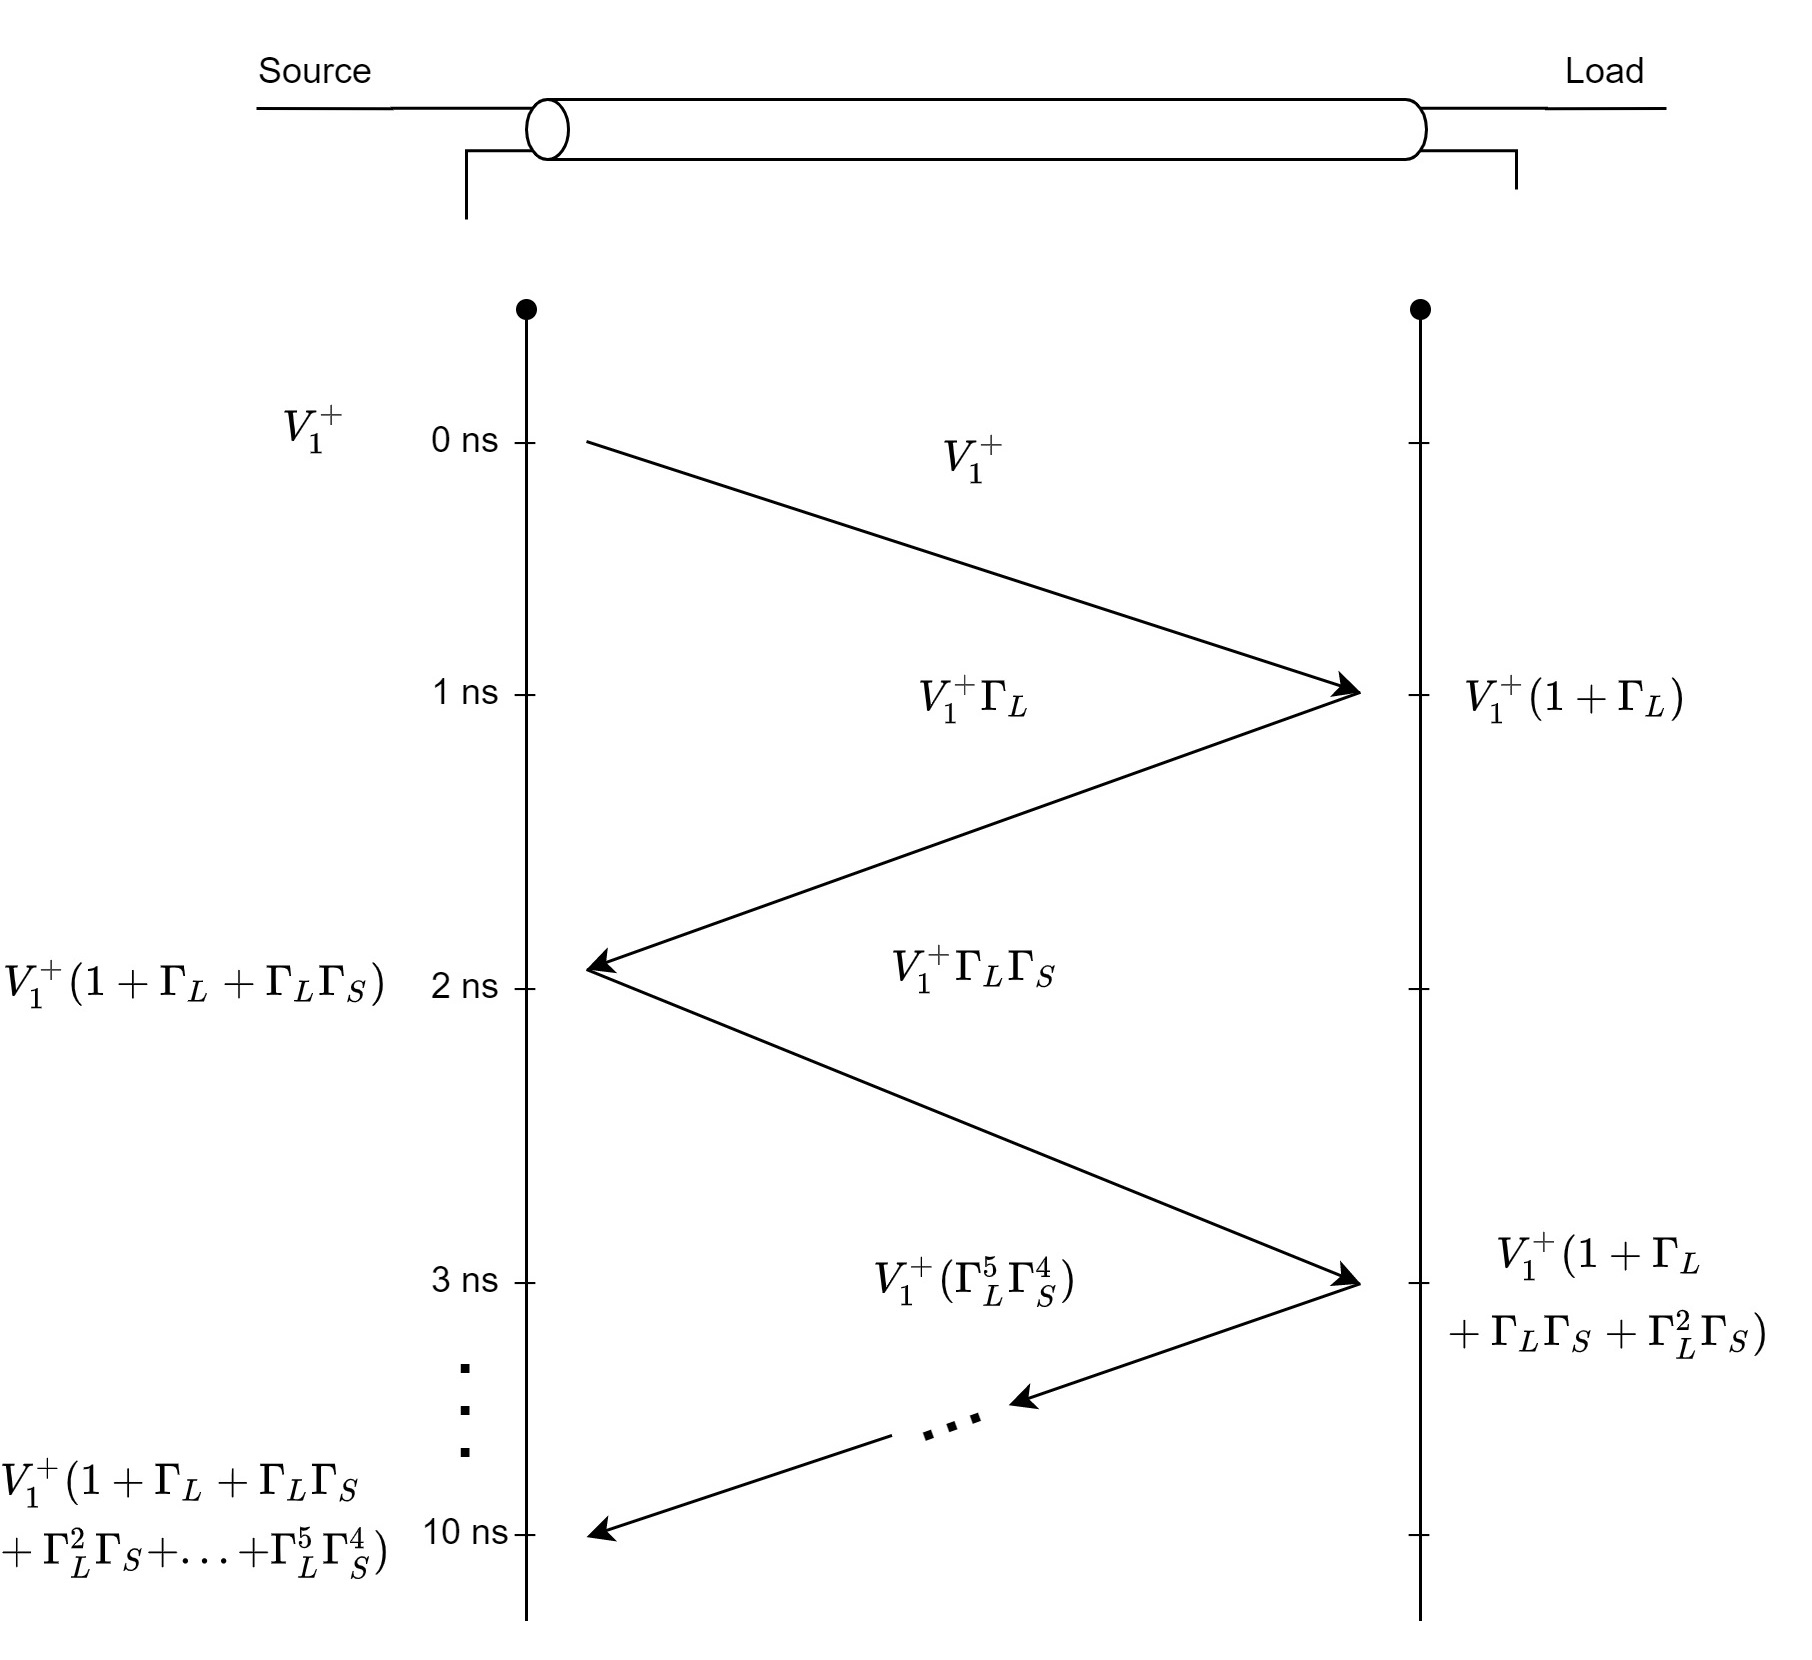
\includegraphics[width=12cm]{images/transient_bouncing_diagram.jpg}
\caption{Transient bouncing diagram for $10ns$. Source: own.}
\label{bouncing} 
\end{figure}

Considering the current source as ideal ($Z_s=\infty$), we can derive the expression for the reflection coefficient at the source \ref{gammaS} and also the reflection coefficient at the load with the load and line characteristic impedance \ref{gammaL}.

\begin{equation} \label{gammaS}
    \Gamma_S = \frac{Z_S - Z_0}{Z_S + Z_0} = \frac{1 - \frac{Z_0}{Z_S}}{1 + \frac{Z_0}{Z_S}} = 1
\end{equation}

\begin{equation} \label{gammaL}
    \Gamma_L= \frac{Z_L - Z_0}{Z_L + Z_0} = \frac{50 - 45}{50 + 45} = \frac{1}{19} 
\end{equation}

Calculating all possible values of voltage across the time in each end of the line with the help of the MATLAB script below we obtain the table \ref{table1}.

\lstinputlisting[language=Matlab,style=mystyle]{matlab/TL.m}

\begin{table}[H]
\centering
\caption{Comparison between datasheet and simulation result for insertion power gain at  $V_{cc} = 3V$ and $I_{cc} = 6mA$,}
\label{table:1}
\begin{tabular}{|c|c|c|}
\hline
\textbf{}                & \multicolumn{2}{c|}{\textbf{Insertion power gain $|s_{21}|^2$ (dB)}} \\ \hline
\textbf{Frequency (MHz)} & \textbf{Datasheet}               & \textbf{Simulation}               \\ \hline
100                      & 25                               & 24.964                            \\ \hline
150                      & 24.5                             & 24.765                            \\ \hline
450                      & 22.5                             & 22.511                            \\ \hline
900                      & 18.5                             & 18.753                            \\ \hline
1500                     & 14.5                             & 14.939                            \\ \hline
1900                     & 12.5                             & 12.939                            \\ \hline
2400                     & 10.5                             & 10.845                            \\ \hline
3500                     & 7                                & 7.054                             \\ \hline
\end{tabular}
\end{table}

From the data above, we conclude that even with impedance mismatch between the load and the line, while waiting some time the voltages will come to equilibrium and the load voltage will behave like there is no line impedance at all. The figure \ref{ads:plot:voltages45} extracted from the simulation on ADS illustrates the voltages behavior.

\begin{figure}[H]
\begin{center}
    \subfigure[MATLAB]{             
        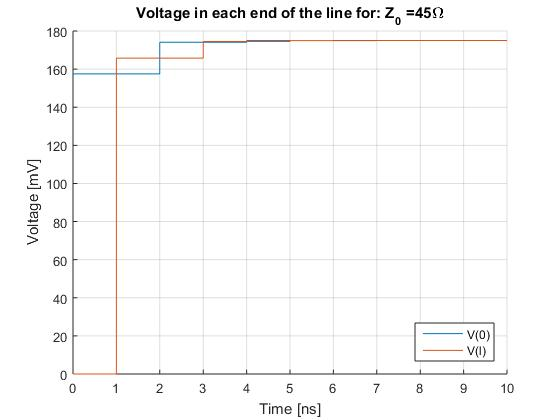
\includegraphics[width=7.5cm]{images/tl_voltage1.jpg}  
        \label{voltages45:1}
    }
    \subfigure[ADS]{                                              
        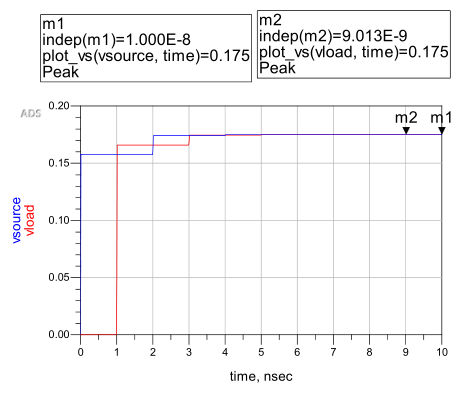
\includegraphics[width=7.5cm]{images/lab1_p1_plot2.png}
        \label{voltages45:2}
    }                
\end{center}
\caption{Plot of voltage values in each end of the line (a) MATLAB and (b) ADS for: $Z_L = 50 \Omega$, $Z_0 = 45 \Omega$ and $Z_S = \infty$.}
\label{ads:plot:voltages45} 
\end{figure}

\subsection{Load voltage waveform for $Z_0=55 \Omega$}

Another test proposes to change the line characteristic impedance to $Z_0=55 \Omega$. Regarding the reflection coeficients, the only one that will change is the one related to the load, so:

\begin{equation} \label{gammaL2}
    \Gamma_L= \frac{Z_L - Z_0}{Z_L + Z_0} = \frac{50 - 55}{50 + 55} = -\frac{1}{21} 
\end{equation}

The same figure \ref{bouncing} of the bouncing diagram and the MATLAB code can be reused (it needs to change de $Z_0$ value in the code).  



\begin{table}[H]
\centering
\caption{Ajustes dos relés de neutro.}
\label{table:2}
\begin{adjustbox}{width=\columnwidth,center}
\begin{tabular}{|l|l|l|}
\hline
\textbf{Parâmetro} & \textbf{Descrição do parâmetro} & \textbf{Ajuste determinado} \\ \hline

RTC & Relação de transformação do TC & 150/5\\ \hline
I (\textit{pickup}) &  Corrente de partida da unidade de tempo inverso de neutro & 6 A\\ \hline
Curva & Curva de atuação da unidade de tempo inverso de neutro & MI-IEC\\ \hline
D.T. & Dial de tempo da unidade de tempo inverso de neutro & 0.2\\ \hline
I def. & Corrente de partida da unidade tempo definido de neutro & 240 A\\ \hline
T def. & Tempo da unidade de tempo definido de neutro & 0.05 s\\ \hline
I inst. & Corrente da unidade instantânea de neutro & 240 A\\ \hline
\end{tabular}
\end{adjustbox}
\end{table}

\begin{figure}[H]
\begin{center}
    \subfigure[MATLAB]{             
        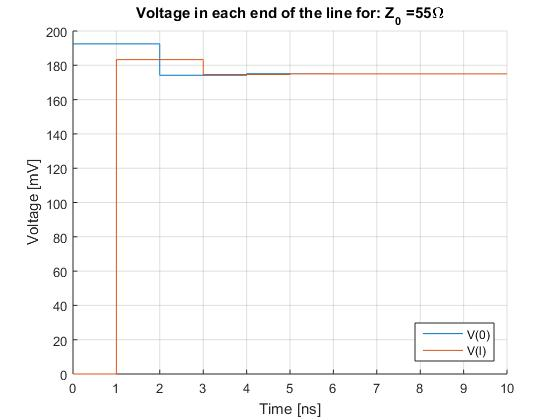
\includegraphics[width=7.5cm]{images/tl_voltage2.jpg}  
        \label{voltages55:1}
    }
    \subfigure[ADS]{                                              
        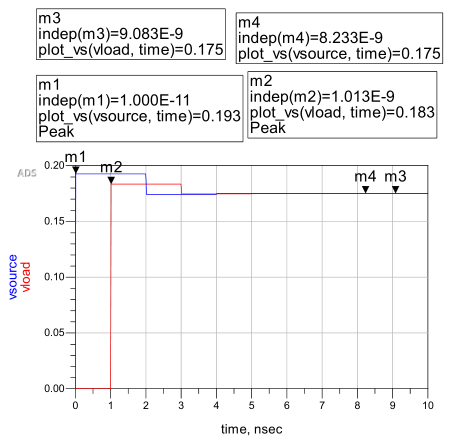
\includegraphics[width=7.5cm]{images/lab1_p1_plot3.png}
        \label{voltages55:2}
    }                
\end{center}
\caption{Plot of voltage values in each end of the line (a) MATLAB and (b) ADS for: $Z_L = 50 \Omega$, $Z_0 = 55 \Omega$ and $Z_S = \infty$.}
\label{ads:plot:voltages55} 
\end{figure}

The results showed in the table \ref{table2} and graphically in the figure \ref{ads:plot:voltages55} allow us to see the effects of the risen in the line characteristic impedance above the load impedance value. The direct effect is an overshoot in the voltage value. Despite this, the voltage values tend to equilibrium just like the previous experiment.

\subsection{Maximum overshoot tolerance in load voltage}

Now considering a receptor input polarized with $1V$ and maximum voltage tolerable of $1.18V$. In the previous topic we have seen that a line characteristic impedance higher than the load impedance provokes a overshoot in the voltage on both ends of the line. The highest peak occurs when the first reflection occurs. So we have to figure it out which value of $Z_0$ guarantees a max. voltage deviation of $0.18 V$.

\begin{center}
    $V_1^+ + V_1^- < \delta_V$ \\ \vspace{1pt}
    $IZ_0 (1+ \Gamma_L) < \delta_V$ \\ \vspace{1pt}
    $IZ_0 \left(1+ \frac{Z_L - Z_0}{Z_L + Z_0}\right)< \delta_V$ 
\end{center}
\begin{equation} \label{maxOS}
    Z_0 < \frac{\delta_V Z_L}{2IZ_L-\delta_V}
\end{equation}

So according to equation \ref{maxOS} for a voltage deviation of $\delta_V = 180 mV$, we can observe that the max. value for the line characteristic impedance is $Z_0 = 52.94 \Omega$. We have obtained the results in the plot of figure \ref{plot:voltages52} that compares the theoretical value in MATLAB with the corresponding simulation on ADS (without the polarization of $1V$).

\begin{figure}[H]
\begin{center}
    \subfigure[MATLAB]{             
        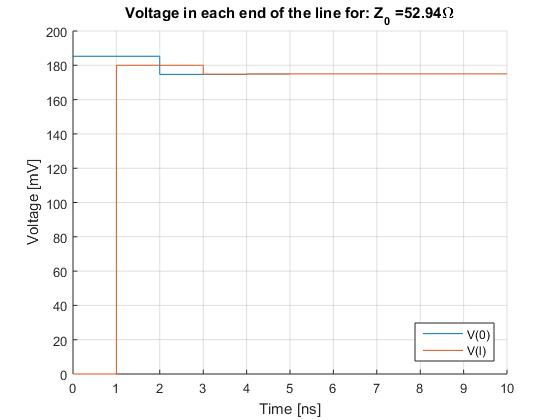
\includegraphics[width=7.5cm]{images/tl_voltage3.jpg}  
        \label{voltages52:1}
    }
    \subfigure[ADS]{                                              
        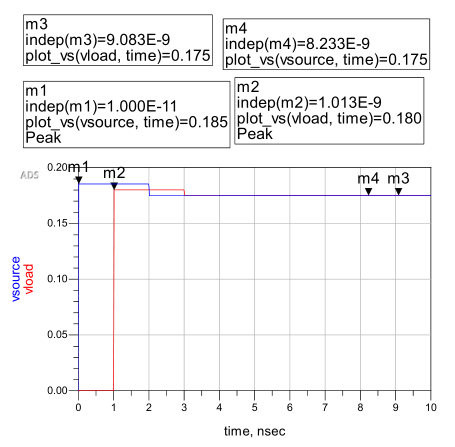
\includegraphics[width=7.5cm]{images/lab1_p1_plot4.png}
        \label{voltages52:2}
    }                
\end{center}
\caption{Plot of voltage values in each end of the line (a) MATLAB and (b) ADS for: $Z_L = 50 \Omega$, $Z_0 = 52.94 \Omega$ and $Z_S = \infty$.}
\label{plot:voltages52} 
\end{figure}